Combining this constraint with a positive relationship of living standards and population growth yields the canonical Malthusian model of stagnation  The importance of this ``Malthusian constraint'' in production can be measured by the elasticity of output with respect to land. Much of the literature, while acknowledging land is necessary, does not concern itself with the specific size of this elasticity, nor consider the possibility that the elasticity may vary across economies. In this paper, we first establish that the quantitative effect of productivity and population on living standards depends on the size of this elasticity. Then, in the main contribution of the paper, we provide estimates of the elasticity across different geographic and political regions. These estimates show significant variation, with a larger elasticity - a ``tighter'' Malthusian constraint - in temperate areas and a smaller elasticity in tropical areas. This in turn implies that living standards are more sensitive to population and productivity shocks in temperate areas, with consequences for subsequent development. 

To establish the importance of the elasticity of agricultural output with respect to land - the ``land elasticity'' hereafter - we provide a static two-sector model of agriculture and non-agriculture with several key features. First, we consider an economy that is made up of many locations, each with its own stock of agricultural land, but where labor and other inputs move freely between locations. This reveals a simple cross-sectional relationship between the density of agricultural workers in a location and agricultural total factor productivity (TFP) that provides us with a specification we can use to estimate the land elasticity. Second, we allow for the presence of factors beyond land and labor (e.g. capital), and show that our estimation strategy does not rely on data on these other inputs. Last, by incorporating an explicit non-agricultural sector and using non-Gorman preferences over agriculture and non-agriculture that allows for non-homotheticity \citep{boppart2014} we are able to derive simple analytical solutions for real income per capita and the share of labor in agriculture. This shows that the elasticity of both outcomes with respect to population and productivity (in either sector) is increasing with the land elasticity. As agriculture becomes more sensitive to the use of land, living standards and the agricultural labor share both become more sensitive to shocks. The intuition is that as agricultural output becomes more sensitive to land, it becomes \textit{less} sensitive to capital and labor, and hence it takes larger movements of those inputs into or out of agriculture to reach equilibrium in response to a change in population or productivity. The implication is that areas with a high land elasticity develop faster in response to positive productivity shocks or drops in population, but also suffer more from population increases and negative productivity shocks.

Theoretically, variation in the land elasticity across economies could be important in explaining comparative development. But does the land elasticity vary at all? To answer that we estimate the land elasticity for different samples of districts (i.e. 2nd level administrative units) from around the world. As noted, our basic specification is taken from the production side of our model, which shows that under mild assumptions the spatial distribution of \textit{agricultural} workers across districts \textit{within} provinces or states is informative about the land elasticity in those districts. Province-level fixed effects capture unobservable information on non-labor inputs, and we do not rely on cross-country comparisons, nor do we have to assume the land elasticity is homogenous within countries. 

All of our estimates come from within-province variation. It is important to note that our specification is derived from only the agricultural production side of our model. The assumptions we made regarding preferences and non-agricultural production are used solely to illustrate the importance of the land elasticity for living standards, and are not relevant for the empirical work.



Further, we are estimating the aggregate production function elasticity for land, and the underlying farm-level production functions that give rise to the factor share data may not share the same elasticity. For agricultural production, this has been discussed since \citet{Hayami:1970ly}, and is an application of \citet{houthakker1955}, where an aggregate Cobb-Douglas may represent the envelope of a set of different techniques, each of which may have an elasticity of substitution between factors different than one (including zero). The factor share information, assuming markets are complete, may provide an accurate estimate of the elasticity of output with respect to land conditional on a fixed technique, but the aggregate elasticity we estimate can differ given the possibility of changing techniques. 


\vspace{.5cm}\noindent\textbf{Measurement Error in rural density:} If there were classical measurement error in rural density, then our estimated $\beta_g$ would be subject to attenuation bias. If one believes the variance of the measurement error is \textit{larger} in tropical areas, such as South-east Asia or tropical Africa, then the estimated elasticity will be attenuated more than in temperate areas, and this could explain the pattern of results we have found. 

The most likely source of this on the population side would seem to be poor census-taking procedures in the countries in tropical regions. We cannot rule this out, but the scale of the measurement error necessary to account for the differences appears extreme. For example, we estimate that $\beta_g$ is almost 0.25 for temperate districts, and approximately 0.125 for tropical districts. For this two-fold difference to have been driven by measurement error in the tropical region, the true variance in (log) rural density would have to be \textit{half} of the measured variance. This in turn would imply that half of the rural densities from HYDE were overstated by a factor of two or more, or understated by a factor of one-half or less. It seems implausible that measurement error in rural density could be this dramatic, and moreover only this dramatic in tropical countries.

More worrisome would be some kind of systematic measurement error in rural density. Given our empirical setting, this would have to be systematic measurement error across districts \textit{within} provinces. And further, the systematic measurement error would have to be present predominantly in either tropical or temperate regions, but not both, in order to account for the results. For example, if within tropical provinces it was the case that relatively dense districts had their density over-reported (and less dense districts had their density under-reported) then it would appear that the correlation of density to agricultural productivity was very large, and hence $\beta_g$ would be estimated to be very small. We cannot rule this out (or the logical opposite of systematic smoothing of rural density counts within temperate provinces), but it is not obvious why such systematic errors would take place \textit{within} provinces but only for one type of climate area. It is not a question of development level, as we are not comparing relatively rich temperate areas to relatively poor tropical areas, but are rather comparing districts within provinces to one another. 

The underlying HYDE data on district-level rural populations is taken from administrative data, not an imputation. As noted above in the robustness sub-section, IPUMS data confirms that the rural data is a strong proxy for agricultural workers, so it is unlikely to be that in tropical areas our rural density is overstating agricultural density in some districts versus others. Also, as mentioned earlier, we can eliminate any district that has a medium-sized urban area located within it, which might perhaps lead to overstatesment of rural density, and our results hold.

\subsection{Results by Political Regions}
Based on the patterns of elasticities seen by crop suitability and climate zone, we would expect that land constraints vary across groups of countries within specific political regions (e.g. Northwest Europe or Southeast Asia). Here we show significant differences in the estimated $\beta_g$ when we group districts by these political regions. In these classifications, we will be forcing all districts within a nation to belong to the same geographic region, and hence have a common $\beta_g$. This obscures variation in agro-climatic conditions within nations. Nevertheless, it is interesting to see how the values of $\beta_g$ vary across political regions, as so much other research on economic development is based on these kinds of regional distinctions, rather than at the agro-climatic level.

Table \ref{TAB_beta_subregion} shows the estimates for fifteen separate regions, the exact definitions of which can be found in the Appendix. We start in Panel A, column (1) with North and Western Europe. The estimated value is 0.259, consistent with column (2), where the estimated value for Eastern Europe is 0.287, and column (3) where the estimated value for Southern Europe is 0.272. We test both of the latter regions against the estimate for Northwest Europe, and cannot reject the hypothesis that they are equal in either case (p-values of 53.9 and 79.1\%). 

Moving to Asia in columns (4) and (5), we have separated the continent into South and Southeastern Asia (which includes India and Indonesia) and Central and West Asia (which includes the Mideast). Neither sub-region includes China, Korea, or Japan, which we will address in Panel C. For South and Southeast Asia, the estimated value of $\beta_g$ is 0.152, lower than in Northwest Europe by about 0.10, similar to the difference between temperate and tropical estimates. We can reject equality with the $\beta_g$ from Northwest Europe (p-value of 1.7\%). For Central and Western Asia the estimated value is 0.181, and this is statistically different from the value in Northwest Europe at 10\% (p-value 7.2\%). The Malthusian constraint appears to be tighter in Europe as a whole when compared to both Asian sub-regions, consistent with the climate and crop regressions presented earlier.

Panel B begins in columns (1) and (2) by showing the result for temperate and tropical countries in the Americas. For temperate countries, the estimated value of $\beta_g$ is 0.188, and given more noise in the estimate we cannot reject equality with the Northwest Europe value, as the p-value is 13.3\%. For the tropical countries of the Americas, the estimated value of $\beta_g$ is only 0.113, and this is different from the Northwest Europe value at less than 0.1\%.

In the remainder of Panel B, we display results for various sub-regions of Africa. In column (3) we have the tropical region spreading across the center of the continent. For this sub-region, the estimated value is 0.089, and significantly lower (at less than 0.1\%) than the Northwest European value. Tropical Africa has the lowest estimated elasticity of any sub-region, even though this area is amongst the poorest and most dependent on agriculture, and is a reminder that the land elasticitiy by itself does not tell us whether the \textit{level} of productivity is high or low. In southern Africa, reported in column (4), the estimated $\beta_g$ is 0.134, similar to the Asian and tropical African values. Given the small sample size, we cannot reject the hypothesis that $\beta_g=0$ (5.9\% p-value) at 5\%, and we cannot reject equality with Northwest Europe at 10\% (11.6\% p-value). For North Africa, in column (5), however, we have a similar estimate to the European ones, at 0.249. We cannot reject equality with the Northwest European value.

The final panel of Table \ref{TAB_beta_subregion} shows results for China, Japan, and the Koreas. We explore the breakdown within China in columns (1) through (3) to demonstrate how significant the differences can be in $\beta_g$ even within countries. Column (1) shows the estimate for China as a whole, yielding an estimate of 0.388, quite high compared to other regions. When we split provinces into temperate and sub-tropical regions (see Appendix for the split by province), however, there appears to be substantial heterogeneity. Column (2) shows that for the temperate provinces, the land elasticity is very high, with $\beta_g$ estimated to be 0.508. But in sub-tropical China the estimated value is only 0.095, similar to the other tropical areas examined in \ref{TAB_beta_subregion}.

Columns (4) and (5) provide estimates for Japan and the Koreas. The estimated values, 0.177 and 0.162 respectively, tend to be closer to the value for sub-tropical China than to temperate China. Compared to other regions explored earlier, these are low compared to areas like Northwest Europe, but equivalent to other tropical areas. These results are consistent with what we found using the agricultural type in Table \ref{TAB_beta_crops}, but appear to run counter to the climate results from Table \ref{TAB_beta_kg}, as neither Japan nor the Koreas fall into equatorial zones with hot summer months. This may suggest that it is the type of crops, rather than the climate conditions themselves, that dictate the size of $\beta$.

Regardless, Table \ref{TAB_beta_subregion} shows that there are significant differences in the tightness of land constraints across regions of the world, whether that is driven by agricultural type or climate. It is notable that some of the poorest areas of the world today, such as tropical Africa, the tropical Americas, and South Asia, exhibit the \textit{loosest} land constraints. It is worth pointing out again that our results here are not driven by comparing rich regions to poor regions, or even rich provinces to poor provinces within countries. With the province level fixed effects, we are using variation in rural density across districts \textit{within} provinces, and information about differences in rural densities across provinces or countries is not used. Our results in Table \ref{TAB_beta_subregion} are not a proxy for income per capita or capital endowments.


\begin{table}[!htb]
\begin{center}
\caption{Estimates of Malthusian Tightness, $\beta$, by K{\"o}ppen-Geiger Zone, 2000CE}
\label{TAB_beta_kg}
{\footnotesize
\begin{tabularx}{\textwidth}{lXXXXXX}
\midrule
\multicolumn{7}{l}{Dependent Variable in all panels: Log caloric yield ($A_{isg}$)} \\ \\
\multicolumn{7}{l}{Panel A: Climate Zones} \\
 & Equatorial & Arid & Temperate & Snow  &     &   \\
 & (1) & (2) & (3) & (4) &  & \\
\midrule
Log rural density   &       0.111&       0.154&       0.169&       0.230\\
                    &     (0.015)&     (0.026)&     (0.017)&     (0.026)\\
\midrule
p-value $\beta=0$   &       0.000&       0.000&       0.000&       0.000\\
p-value $\beta=\beta^{Equa}$&            &       0.151&       0.007&       0.000\\
Countries           &          79&          56&          94&          40\\
Observations        &       11461&        2822&       13717&        6327\\
Adjusted R-square   &        0.11&        0.10&        0.15&        0.19\\

\midrule
\\
\multicolumn{7}{l}{Panel B: Precipitation Zones} \\
& Fully     & Dry         & Dry        &              &            & \\
& Humid & Summer & Winter & Monsoon & Desert & Steppe \\
 & (1) & (2) & (3) & (4) & (5) & (6) \\
\midrule
Log labor/land ratio ($\beta_g$)&       0.240&       0.215&       0.124&       0.125&       0.130&       0.147\\
                    &     (0.044)&     (0.063)&     (0.022)&     (0.039)&     (0.072)&     (0.029)\\
\midrule
p-value $\beta=0$   &       0.000&       0.001&       0.000&       0.001&       0.072&       0.000\\
p-value $\beta=\beta_{Humid}$&            &       0.739&       0.020&       0.043&       0.190&       0.072\\
Countries           &          78&          37&          67&          32&          20&          49\\
Observations        &       13545&        2373&        7695&        1267&         146&        1735\\
R-square (ex. FE)   &        0.17&        0.17&        0.15&        0.17&        0.17&        0.16\\

\midrule
\\
\multicolumn{7}{l}{Panel C: Temperature Zones} \\
    & Hot        & Warm        & Cool       & Hot      & Cold     &  \\
    & Summer & Summer & Summer & Arid & Arid &   \\
 & (1) & (2) & (3) & (4) & (5) &  \\    
\midrule
Log labor/land ratio ($\beta_g$)&       0.142&       0.226&       0.207&       0.140&       0.190\\
                    &     (0.021)&     (0.053)&     (0.076)&     (0.035)&     (0.046)\\
\midrule
p-value $\beta=0$   &       0.000&       0.000&       0.007&       0.000&       0.000\\
p-value $\beta=\beta_{Humid}$&            &       0.065&       0.405&       0.969&       0.254\\
Countries           &          57&          82&          18&          42&          25\\
Observations        &        8101&        9003&         340&        1230&         956\\
R-square (ex. FE)   &        0.20&        0.23&        0.20&        0.17&        0.21\\

\midrule
\end{tabularx}
}
\end{center}
\vspace{-.5cm}\singlespacing {\footnotesize \textbf{Notes}: Conley standard errors, adjusted for spatial auto-correlation with a cutoff distance of 500km, are shown in parentheses. All regressions include province fixed effects, a constant, and controls for the district urbanization rate and log density of district nighttime lights. The coefficient estimate on rural population density indicates the value of $\beta_g$, see equation (\ref{EQ_regress}). Rural population is from HYDE database \citep{hyde31}, and caloric yield is the author's calculations based on the data from \citet{galorozak2016}. Inclusion of districts is based on whether they have more than 50\% of their land area in the given K{\"o}ppen-Geiger zone. See text for details.
}
\end{table}

\clearpage
\begin{table}[!htb]
\begin{center}
\caption{Estimates of Malthusian Tightness, $\beta$, by Regions, 2000CE}
\label{TAB_beta_subregion}
{\footnotesize
\begin{tabularx}{\textwidth}{lXXXXX}
\midrule
\multicolumn{6}{l}{Dependent Variable in all panels: Log caloric yield ($A_{isg}$)} \\ \\
\multicolumn{6}{l}{Panel A} \\
 &          &         &             &  \multicolumn{2}{c}{Excl. China, Japan, Korea} \\ \cmidrule(lr){5-6}
 & North \& &         &              & South \&  & Central \&             \\
 & Western  & Eastern & Southern     & Southeast & West        \\
 & Europe   & Europe  & Europe       & Asia      & Asia      \\
 & (1) & (2) & (3) & (4) & (5) \\
\midrule
Log rural density ($\beta_g$)&       0.259&       0.287&       0.272&       0.152&       0.181\\
                    &     (0.036)&     (0.031)&     (0.041)&     (0.026)&     (0.024)\\
\midrule
p-value $\beta=0$   &       0.000&       0.000&       0.000&       0.000&       0.000\\
p-value $\beta=\beta_{NWEur}$&            &       0.539&       0.791&       0.017&       0.072\\
Countries           &          16&           9&           9&          13&          18\\
Observations        &        1684&        4821&        1137&        4312&        2878\\
R-square (ex. FE)   &        0.29&        0.34&        0.32&        0.21&        0.24\\

\midrule
\\
\multicolumn{6}{l}{Panel B} \\
 & Temperate & Tropical  & Tropical & South    & North    \\
 & Americas  & Americas  & Africa   & Africa   & Africa     \\
\midrule
Residuals           &       0.188&       0.113&       0.089&       0.134&       0.249\\
                    &     (0.030)&     (0.016)&     (0.014)&     (0.071)&     (0.014)\\
\midrule
p-value $\beta=0$   &       0.000&       0.000&       0.000&       0.059&       0.000\\
p-value $\beta=\beta_{NWEur}$&       0.133&       0.000&       0.000&       0.116&       0.827\\
Countries           &           5&          22&          39&           4&           5\\
Observations        &        3796&        9373&        3181&         198&        1220\\
R-square (ex. FE)   &        0.24&        0.12&        0.18&        0.27&        0.28\\

\midrule
\\
\multicolumn{6}{l}{Panel C} \\
 & All& Temperate & Sub-Tropical & & North \& \\
 & China & China  & China & Japan & South Korea  \\
 & (1) & (2) & (3) & (4) & (5) \\
\midrule
Log rural density   &       0.414&       0.518&       0.107&       0.155&       0.190\\
                    &     (0.083)&     (0.058)&     (0.026)&     (0.011)&     (0.061)\\
\midrule
p-value $\beta=0$   &       0.000&       0.000&       0.000&       0.000&       0.002\\
p-value $\beta=\beta^{NWEur}$&       0.102&       0.000&       0.001&       0.008&       0.309\\
Countries           &           1&           1&           1&           1&           2\\
Observations        &         266&         130&         136&        1039&         311\\
Adjusted R-square   &        0.25&        0.26&        0.21&        0.21&        0.21\\

\midrule

\end{tabularx}
}
\end{center}
\vspace{-.5cm}\singlespacing {\footnotesize \textbf{Notes}: Conley standard errors, adjusted for spatial auto-correlation with a cutoff distance of 500km, are shown in parentheses. All regressions include province fixed effects, a constant, and controls for the district urbanization rate and log density of district nighttime lights. See appendix for lists of exact countries included in each region. The coefficient estimate on rural population density indicates the value of $\beta_g$, see equation (\ref{EQ_regress}). Rural population is from HYDE database \citep{hyde31}, and caloric yield is the author's calculations based on the data from \citet{galorozak2016}. The countries included in each region can be found in the appendix.
}
\end{table}


A related issue would be if the HYDE database incorrectly mapped rural population data into districts, or if we have made errors in how we assigned HYDE grid cells to districts in aggregating the data. To address this, in the Appendix we have re-estimated all of our results at the province/state level (and using country fixed effects), where the likelihood of both kinds of assignment errors is smaller, given the smaller number of borders, and the smaller weight that any given grid-cell would have in a larger political unit. At this level, the pattern of our results is identical. The only difference is that the estimated elasticities for the temperate samples are somewhat \textit{higher}, indicating larger differences between temperate and tropical regions.\footnote{In the Appendix, we also show that our results are consistent if we use an alternative source of grid-cell level population data \citep{grump2011}.}

\subsection{Results by Climate Zone}
The temperate versus tropical distinction depends in large part on climatic characteristics, and in this section we look at how the value of $\beta_g$ is related to specific climates. For this, we use the K{\"o}ppen-Geiger scheme, which classifies each grid cell on the planet on three dimensions \citep{kottek2006}. First are the \textit{main climate} zones: equatorial (denoted with an ``A''), arid (B), warm temperate (C), and snow (D).\footnote{There is another classification of climate, polar (E), but that covers only areas that are uninhabited for all intents and purposes.} Second, each grid-cell has a \textit{precipitation} classification: fully humid (f), dry summers (s), dry winters (w), monsoonal (m), desert (D), and steppe (S). Finally, there is the \textit{temperature} dimension: hot summers (a), warm summers (b), cool summers (c), hot arid (h), and dry arid (k).\footnote{There are three other temperature classifications - extreme continental, polar frost, and polar tundra - that also cover only uninhabited areas.} Each grid cell thus receives either a three or two-part code. The area around Paris, for example, is ``Cfb'', meaning it is a warm temperate area, fully humid (rain throughout the year), with warm summers. The area near Saigon is ``Aw'', meaning it is equatorial, with dry winters. There is no separate temperature dimension assigned to equatorial zones, as it tends to be redundant.

What we do in Table \ref{TAB_beta_kg} is divide districts into regions based on their K{\"o}ppen-Geiger classifications, as opposed to crop suitability or production data. We do this along each individual dimension (climate, precipitation, and temperature), including a district in a region if more than 50\% of its land area falls in the given zone. For example, for the equatorial region, we include all districts in which 50\% (or more) of their land area is classified as being in ``A'' in the K{\"o}ppen-Geiger system, regardless of their precipitation or temperature codes. Narrowing down to very specific classifications (``Cfb'', for example) is impractical because the number of districts becomes very small. Similar to the temperate/tropical regressions, the climate zone regions do not force heterogeneous districts to be lumped into single regions based on their nation. 

In Panel A of Table \ref{TAB_beta_kg} we show the results for the different climate zones. The land elasticity in equatorial zones is estimated to be 0.111, similar in size to what we saw for areas suitable for tropical agriculture. The arid zone has an estimate of 0.154, and then the estimated elasticities become higher. The warm temperate zone has an estimated elasticity of 0.169, while the snow zone has a coefficient of 0.230. Based on these results, the Malthusian constraint becomes tighter as climates become cooler. This is consistent with the agriculture results. Both temperate and snow climate estimates of $\beta_g$ are significantly different from the equatorial value, with p-values of 0.7\% and less than 0.1\%, respectively.

Panel B shows the estimates when we create regions based on their precipitation regime. Here, we can see that the first two types - fully humid and dry summers - both have estimated land elasticities that are large, at 0.185 and 0.169, and we cannot reject that these values are identical (p-value of 0.594). Fully humid areas are those with year-round rain, and dominate the eastern U.S., Western Europe, the River Plate basin, the east coast of Australia, Indonesia, and the sub-tropical areas of China. The dry summer areas are associated with Mediterranean climates, as well as with the west coast of the United States, Chile, and some central areas of India.

Places with dry winters (column 3), or which rely on monsoons (column 4) have estimated elasticities of 0.115 and 0.130, respectively. These areas cover the majority of the equatorial regions of the world, from the Amazon basin, across central Africa, and envelope nearly all of south and south-east Asia. The difference of the dry winter constraint from the fully humid constraint is significant (1.3\%), while the monsoon value is significantly different at 9\%. The final two precipitation regimes are deserts and steppe areas, which are estimated to have even looser land elasticities than the others, at 0.112 and 0.110, but due to smaller sample sizes the differences with fully humid districts are not all significant (i.e. a p-value of 12\% for Desert districts).

The final panel of Table \ref{TAB_beta_kg} shows the results from regions based on temperature zones. Districts with hot summers, in column (1), have an estimated constraint of 0.142. In columns (2) and (3), places with warm or cool summers have much tighter land constraints, estimated at 0.219 and 0.247, respectively. These are both significantly different from the value for districts with hot summers (0.4\% and 3.5\%). In comparison, the arid areas, whether hot or cold, in columns (4) and (5), show lower estimated elasticities, and the difference with hot summer regions cannot be rejected (85.0 and 57.6\% p-values).

While we have separated the districts according to single dimensions, each area is composed of a set of these characteristics. The individual estimates in Table \ref{TAB_beta_kg} would interact to create the exact land elasticity in each individual district or province. While there may be non-linear effects at work, one can see some logic in simple averages across the different types of climate zone. For example, places that are in the ``snow'' climate zone (0.230), with ``fully humid'' precipitation (0.185), and with ``warm summers'' (0.219), should tend to have high land elasticities and tight Malthusian constraints. Places like this include southern Canada and the upper Midwest in the United States, and much of eastern Europe and western Russia. These are also places that practice temperate agriculture. In contrast, districts in equatorial areas (0.111), with dry winters or monsoons (0.115-0.130), regardless of temperature regime, have relatively low elasticities and loose Malthusian constraints.

\subsection{Historical Implications}
While we cannot perform as robust of a test as with the epidemiological transition, our estimates of $\beta$ offer a way to understand several issues in historical development. In Europe, the Black Death had a substantial positive effect on living standards and urbanization, and it has been proposed that this had persistent effects on development \citep{vv08,vv13}. Similar epidemics also hit regions of Asia, without appearing to have initiated such fundamental changes \citep{McNeill1976}. Proposition 1 suggests that the reason for this subdued response could be the looser land constraint found in Asia, which muted the transition of labor out of agriculture and the increase in living standards. 

Leaving aside epidemics, Asian development has often been characterized by ``involution'' \citep{Geertz1963,Huang1990,huang2002}, where technological changes occurred, but led to higher density without higher living standards or urbanization. Proposition 1 showed that the loose land constraint may be a source of involution, by muting the response of Asian economies to productivity shocks, and requiring them to experience greater productivity improvements just to keep up with regions having tight land constraints (e.g. Europe). The high historical population density in Asia relative to Europe can also be understood in terms of the land elasticity. If one adds a Malthusian fertility response on top of our model here (see Appendix), it can be shown that the elasticity of equilibrium population size with respect to productivity is \textit{decreasing} with the land elasticity. Similar percent increases in productivity in Asia would result in larger percent increases in population density than in Europe. Over time their density would rise relative to Europe even if they had no advantage in the rate of productivity growth.

From a more contemporary perspective, areas that developed more rapidly (east Asia) tend to have tighter land constraints than those who lagged behind (tropical Africa, central America). As with involution, the results here suggest why that may be the case, as the loose land constraints in Africa and Central America would restrict their gains from realized productivity gains, and require more growth in productivity just to keep pace over time. 



To illustrate the essence of our results, Figure \ref{FIG_beta_crop} plots the raw data on (log) caloric yield, $A_{isc}$ against (log) rural density, $L_{isc}/X_{isc}$ for two sets of districts. The first are those districts that have a suitability index for wheat that is greater than zero, but for which their suitability for rice is zero. In the figure, these data points are plotted in black, with the simple bivariate OLS fitted line plotted. As one can see, there is a positive slope between density and productivity, and as per our equation (\ref{EQ_regress}), this slope provides an estimate of $\beta$ for these wheat-capable districts. In comparison, the data points plotted in gray (green if viewed in color) are those districts that have a suitability for rice production that is positive, but have zero suitability for wheat. Again, the bivariate OLS fitted line is plotted, and as can be seen it has a much shallower slope than in the wheat case, and thus a much lower estimated $\beta$.

This simple comparison illustrates the difference between these kinds of districts. Wheat-growing districts display a much tighter Malthusian constraint. Note that rice districts have, on average, much higher caloric yields than wheat areas, in part due to rice's superior number of calories for a given dry weight. But notice that rural densities are very \textit{low} in rice-capable districts that are only \textit{slightly} less productive than those with the maximum. This is the effect we would expect if the land constraint was loose in rice-capable areas.

To make the relationships in Figure \ref{FIG_beta_crop} more concrete, we examine those same relationships in regressions that include province fixed effects, and for varying sub-samples, as in equation (\ref{EQ_regress}). We create the sub-samples of districts based on the crop suitability and/or production data. We will thus be selecting some, but not necessarily all, of the districts of a country into each sample. For example, when we examine a sample that is capable of growing wheat (and other temperate crops), but not rice (or other sub-tropical crops), we will be selecting districts from northern China, but not southern China. Note that this procedure alleviates the issue of assigning a country like the U.S. or Brazil a single biogeographic type.

Panel A selects samples based on the predominant crops that are capable of being grown. A classic comparison is ``wheat vs. rice'' agricultural systems, but each system encompasses a variety of other crops that thrive in similar agro-climatic conditions. We thus define the \textbf{Wheat Family} to include barley, buckwheat, rye, oats, and white potatoes, along with wheat. We define the \textbf{Rice Family} to include cassava, cowpeas, pearl millet, sweet potatoes, and yams, as well as paddy rice. The GAEZ measures of suitability for the crops within a family are all highly correlated. We have experimented with alternative sets of crops in each family, without changing our main results. 

The use of the terms Wheat Family and Rice Family are for convenience, and do not imply that we are estimating the production function \textit{for wheat} or \textit{for rice}, or any of the other crops listed in each family. We are using the crop suitability and production data to identify samples of districts that share common agro-climatic constraints, and estimating the aggregate value of $\beta$ for those agro-climatic zones.

\clearpage


\begin{figure}[!htb]
\begin{center}
\caption{Caloric Yield and Rural Density, by Major Crop, 2000CE}
\label{FIG_beta_crop}
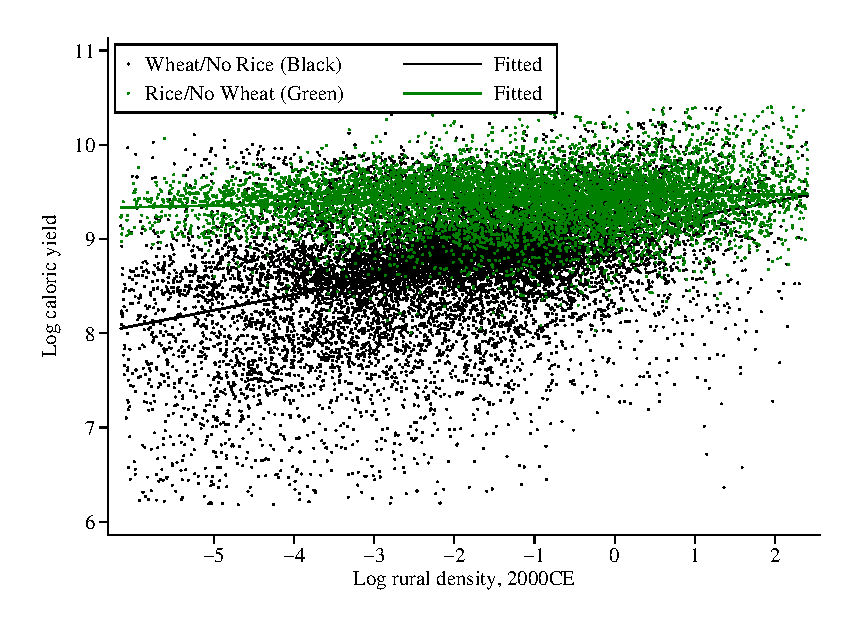
\includegraphics[width=1.0\textwidth]{fig_beta_crop.eps}
\end{center}
\vspace{-.5cm}\singlespacing {\footnotesize \textbf{Notes}: This figures shows the raw correlation of (log) caloric yield and (log) rural density for districts that are (a) suitable for wheat, but not for wet rice, and (b) suitable for wet rice but not for wheat. Rural population is from HYDE database \citep{hyde31}, and caloric yield is the author's calculations based on the data from \citet{galorozak2016}. The linear fits are from bivariate OLS regressions, without any fixed effects included. Based on equation (\ref{EQ_regress}), the slopes of these lines are estimates of $\beta$, the elasticity of agricultural output with respect to land.
}
\end{figure}


//////////////////////////////////////
// Create residual plot of baseline results
//////////////////////////////////////

qui reg ln_csi_yield urb_perc_2000 ln_light_mean i.state_id if dry_suit>0 & wet_suit==0, cluster(state_id)
predict csi_res_dry, res
qui reg ln_rurd_2000 urb_perc_2000 ln_light_mean i.state_id if dry_suit>0 & wet_suit==0, cluster(state_id)
predict rurd_res_dry, res

qui reg ln_csi_yield urb_perc_2000 ln_light_mean i.state_id if dry_suit==0 & wet_suit>0, cluster(state_id)
predict csi_res_wet, res
qui reg ln_rurd_2000 urb_perc_2000 ln_light_mean i.state_id if dry_suit==0 & wet_suit>0, cluster(state_id)
predict rurd_res_wet, res


scatter csi_res_dry rurd_res_dry if dry_suit>0 & wet_suit==0 & ln_csi_yield>0, msymbol(p) mcolor(black) ///
	|| lfit csi_res_dry rurd_res_dry if dry_suit>0 & wet_suit==0 & ln_csi_yield>0, clcolor(black) ///
	|| scatter csi_res_wet rurd_res_wet if dry_suit==0 & wet_suit>0, msymbol(p) mcolor(green) ///
	|| lfit csi_res_wet rurd_res_wet if dry_suit==0 & wet_suit>0, clcolor(green) ///
	xtitle("Residual log rural density, 2000CE") ytitle("Residual log caloric yield") ///
	ylabel(, angle(0) nogrid) graphregion(color(white)) /// xlabel(-5(1)2) ///
	legend(ring(0) pos(10) label(1 "Temperate (Black)") label(2 "Fitted") label(3 "Tropical (Green)") label(4 "Fitted"))
graph export "$output/fig_beta_crop.png", replace as(png)
graph export "$output/fig_beta_crop.eps", replace as(eps)

	


More broadly, HYDE's methodology of mapping of rural population may be driving our results. To assess this, we use a separate data source from the Global Rural-Urban Mapping Project (GRUMP), developed by \cite{Balketal2006}. This project also provides grid-cell level population counts, as well as ``urban masks'' that define cells within urban agglomerations. We extract the count of rural population in a given district from GRUMP as the count of population in all grid cells that are \textit{not} part of urban agglomerations. GRUMP's implicit rural population, then, will not necessarily conform to census reports of rural population (in principle, HYDE's count of rural population should conform). In the Appendix we show results using GRUMP's population data to measure rural density, and the results are consistent with the results from HYDE. There is one exception, which is that when we distinguish samples by their harvested area of crops, the estimated $\beta$ values are no longer statistically different between wheat and rice families. 

Combining this constraint with a positive relationship of living standards and population growth yields the canonical Malthusian model of stagnation \citep{ashraf2010dynamics}, and forms the basis for models of the transition from stagnation to sustained growth. The literature on the transition has grown large enough that it is difficult to provide a reasonable summary in a footnote. An overview of this unified growth literature can be found in \citet{Galor:2011uq}, who cites several key contributions \citep{gw00,galor2002natural,Hansen:2002fk,doepke2004accounting,cs2005,lagerlof2006,craftsmills2009,strulik2008population}. Explanations for the Great Divergence in income per capita are often framed in terms of these unified growth models \citep{kp2001,galor2008trading,vollrath2011,vv08,vv13,cs2015}. The Malthusian constraint features in quantitative work on contemporary developing countries that rely on agriculture \citep{Gollin:2007oq,Restuccia:2008hc,weilwilde2009,Gollin:2010ys,ev2016clim}, and is relevant for long-run growth in relatively rich countries due to possible limits to resources \citep{perettovalente2015}.